% subdivision.tex
% ------------------------------------------------------------------------

\begin{figure}[tb]
  \centering
  \psfrag{A}[]{(a)}
  \psfrag{B}[]{(b)}
  \psfrag{C}[]{(c)}
  \psfrag{D}[]{(d)}
  \epsfig{file=figs/RefMap.eps, width=7cm}
  \caption{The stencil (weights are not shown) and its 
           vertex in the Catmull-Clark subdivision (a-c)
           and Doo-Sabin subdivision (d). Catmull-Clark
           subdivision has three stencils: facet-stencil (a), 
           edge-stencil (b) and vertex-stencil (c). 
           Doo-Sabin subdivision has only corner-stencil (d).}
  \label{fig:RefMap}\vspace*{-4mm}
\end{figure}


%Subdivision surfaces \cite{cc,ds,loop,sqrt3,qts}
%are the limit surface resulting from the
%application of a subdivision algorithm to a control mesh.
%Subdivision algorithms recursively \emph{refine} (subdivide) the
%control mesh and \emph{modify} (smooth) the geometry according
%to a stencil on the source mesh.  
%Further details on subdivisions can be found at \cite{Sub:course:2000}
%and \cite{Warren:subdivision}. The OpenMesh library has
%supports of Loop and $\sqrt{3}$ subdivisions \cite{Abhijit:2004:APISUB}.

Subdivision algorithms \cite{Warren:subdivision, Sub:course:2000} 
contain two major steps: \emph{\tr} and \emph{\gm}.
The \tr\ reparameterizes the control mesh into a refined 
mesh. The \gm\ transforms a submesh on the control mesh
to a vertex on the refined mesh. The submesh (with
the normalized weights) is called the
\emph{stencil}. A subdivision algorithm recursively 
applies these two steps and approximates the limit surface. 
%A proper combination of a \tr\ and a set of 
%rules of \gm\ define a valid subdivision scheme.

The topological refinement is illustrated 
in Fig.~\ref{fig:RefSchemes} for Catmull-Clark
subdivision (PQQ) \cite{cc}, Loop subdivision (PTQ) \cite{loop},
Doo-Sabin subdivision (DQQ) \cite{ds}, and $\sqrt{3}$ subdivision
\cite{sqrt3}. Subdivisions, such as Quad-Triangle subdivision 
\cite{qts,l-pg-03}, may employ a hybrid refinement consisting
of two different refinements.

The \gm\ is illustrated with examples of the correspondence between
stencil and its vertex in Fig.~\ref{fig:RefMap}, where Catmull-Clark
subdivision has three distinct stencils and Doo-Sabin subdivision has
only one stencil. 

\begin{figure}
    \centering{\includegraphics[width=7.0cm]{figs/sqrt3}}
    \caption{$\sqrt{3}$-Subdivision of the mannequin mesh.}
    \label{fig:sqrt3}\vspace*{-3mm}
\end{figure}



%\subsubsection{Sqrt 3}
% connectivity ops: specific polyhedron algorithms (sqrt3 subdivisions) 
\newcommand{\mySqrt}{$\sqrt{3}$}
\subsubsection*{Sqrt-3 Subdivision using Euler Operators}
\input sqrt3

% templated rules: a generic framework for subdivisions 
\subsubsection*{Generic Subdivision Solution}
%\label{sec:subtempl}
\input subtempl


% inc builder: specific polyhedron algorithms (qt subdivisions) 
%\subsection{Quad-triangle Subdivision using modifier}
%\input qt

